\documentclass[12pt]{article}
\usepackage{stata}
\usepackage{graphicx}
\usepackage{geometry}
\usepackage{rotating}
\begin{document}
\author{Jesús Lara Jáuregui}
\title{Problem Set 1}
\maketitle
\section{Problem One. OLS in MATA}
\subsection{Part 1}
In this problem I created the program e-class program myreg1. This program takes as input a dependent variable $y$ and a set of independent variables or regressors $X_k$. The program transform these variables into a vector and matrix respectively and performs the operations necessary to get our OLS estimates and the associated variance-covariance matrix. the output is thus a $b_{(k+1)x1 vector}$ (OLS estimates)  and a $V_(k+1)x(k+1)$ matrix (Variance-covariance).

The log below shows that the results of myreg1 are the same as those obtained using Stata's embed
\ Results with myreg1
\begin{stlog}. myreg1 lnwage hieduc exp exp2 
{\smallskip}
b[4,1]
            c1
r1   .08264541
r2   .02523881
r3  -.00037668
r4   1.3094414
{\smallskip}
symmetric V[4,4]
            c1          c2          c3          c4
r1   1.195e-06
r2   1.595e-07   .00001683
r3  -4.035e-09  -3.770e-07   8.579e-09
r4  -.00001749  -.00017676   3.899e-06   .00211062
{\smallskip}
\end{stlog}
\ Results with Stata OlS command
\begin{stlog}. quiet reg lnwage hieduc exp exp2
{\smallskip}
. matrix list e(b)
{\smallskip}
e(b)[1,4]
        hieduc         exp        exp2       _cons
y1   .08264541   .02523881  -.00037668   1.3094414
{\smallskip}
. matrix list e(V)
{\smallskip}
symmetric e(V)[4,4]
            hieduc         exp        exp2       _cons
hieduc   1.195e-06
   exp   1.595e-07   .00001683
  exp2  -4.035e-09  -3.770e-07   8.580e-09
 _cons   -.0000175  -.00017676   3.899e-06   .00211066
{\smallskip}
\end{stlog}
\begin{table}[htbp]\centering
\caption{Estimates of FB}
\begin{tabular}{l*{8}{c}}
\hline\hline
                    &   Bivariate&      Simple&   Saturated&         CEM&      PScore&   Psmatch\_1&         Own&         IPW\\
\hline
\hline
FB                  &      -0.056&       0.056&            &       0.050&      -0.077&       0.006&       0.125&       0.123\\
                    &     (0.011)&     (0.014)&            &     (0.015)&     (0.116)&     (0.032)&     (0.012)&     (0.142)\\
Obs.                &       51816&       51816&       48626&       37081&       65741&       51816&       51816&       51816\\
Estimator           &OLS Bivariate&OLS Controls&OLS Saturated&         CEM&       Match&       Match&       Match&       Match\\
\hline\hline
\multicolumn{9}{l}{\footnotesize Standard errors in parentheses}\\
\multicolumn{9}{l}{\footnotesize Average Treatment On Treated for matching models}\\
\end{tabular}
\end{table}

\subsection{Part 2}
\pagebreak
In this part I created the program myreg2 which takes the same inputs as myreg1 and gives the same vector of OLS estimates $b$. myreg2 takes the variables from Stata and then implements a second program called myols(X,Y), which is the one that actually calculates the OLS estimates and the variance-covariance Matrix $V$ adjusted for arbitrary heteroscedasticity. With respect to the OLS estimates, instead of calculating them with the cross product (and inverse) of the whole $X$ matrix and $y$ vector, it performs the sum of the cross product of each row (observations). The same approach is used for calculating the matrix $V$.

The log below shows that my results are exactly the same as those obtained using Stata's regress command and "robust" option. 

\begin{stlog}. hist(num_awards), title("Number of Awards") color("orange")
(bin=14, start=0, width=.42857143)
{\smallskip}
\end{stlog}
\ Results with Stata's OLS and robust standard errors
\begin{stlog}. 
. matrix list e(b)
{\smallskip}
e(b)[1,4]
        hieduc         exp        exp2       _cons
y1   .08264541   .02523881  -.00037668   1.3094414
{\smallskip}
. matrix list e(V)
{\smallskip}
symmetric e(V)[4,4]
            hieduc         exp        exp2       _cons
hieduc   1.520e-06
   exp   1.712e-07   .00001632
  exp2  -4.045e-09  -3.685e-07   8.451e-09
 _cons  -.00002216  -.00016979   3.771e-06   .00208194
{\smallskip}
. 
\end{stlog}
\pagebreak

\section{Problem 2. Poisson using Maximum Likelihood}

If $y_i$ is distributed Poission with mean $exp(X^{'}_i \beta)$, hence the likelihood function for a sample of $N$ observations is given by:

$$ L(\beta)=\prod_{i=1}^{N}\frac{1}{y_{i}!}exp((X^{'}\beta)y_i)exp(-exp(X^{'}\beta))$$


And taking logs we get:

$$lnL(\beta)=\sum_{i}^{N}[-exp(X^{'}\beta)+y_i exp(X^{'}\beta)-ln(y_i !)]$$

Which is the form we use for pur maximum-likelihood estimation
I made two .ado files, one containing the generation of the evaluator program and the other one that takes a dependent and independent variables from Stata and performs the Maximum Likelihood Estimation. Those .aso files are attached in the folder. 

I show the histogram of the number of awards as well as the mean and variance of the variable. The key assumption of Poisson distribution is that the parameter $\lambda$ is the mean and variance of y. However, we see that the variance is almost twice bigger than the mean, which may reduce the usefulness of Poisson distribution to analyze the behavior of the number of awards. 

\begin{stlog}. hist(num_awards), title("Number of Awards") color("or
> ange")
(bin=14, start=0, width=.42857143)
{\smallskip}
\end{stlog}
\begin{center}
    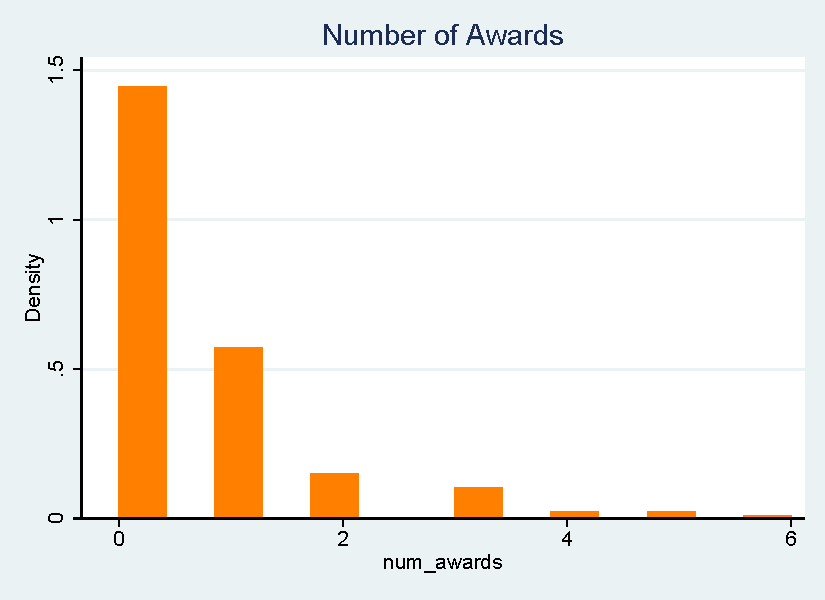
\includegraphics{797B_PS1_JL_5.pdf}
\end{center}
In the table below I show the results of the estimation using Stata's command and mypois. I get the same results.
\begin{table}[htbp]\centering
\caption{Number of Awards}
\begin{tabular}{l*{2}{c}}
\toprule
            &        Mean&    Variance\\
\midrule
Number of awards&        0.63&        1.11\\
\bottomrule
\end{tabular}
\end{table}

\begin{table}[htbp]\centering
\def\sym#1{\ifmmode^{#1}\else\(^{#1}\)\fi}
\caption{Poisson Estimation}
\begin{tabular}{l*{2}{c}}
\hline\hline
                &\multicolumn{1}{c}{(1)}&\multicolumn{1}{c}{(2)}\\
                &\multicolumn{1}{c}{Stata Poisson}&\multicolumn{1}{c}{mypois}\\
\hline
main            &                  &                  \\
general         &   0.0000         &   0.0000         \\
                &      (.)         &      (.)         \\
[1em]
academic        &   1.0839\sym{**} &   1.0839\sym{**} \\
                & (0.3583)         & (0.3583)         \\
[1em]
vocation        &   0.3698         &   0.3698         \\
                & (0.4411)         & (0.4411)         \\
[1em]
math score      &   0.0702\sym{***}&   0.0702\sym{***}\\
                & (0.0106)         & (0.0106)         \\
[1em]
Constant        &  -5.2471\sym{***}&  -5.2471\sym{***}\\
                & (0.6585)         & (0.6585)         \\
\hline
Observations    &      200         &      200         \\
\hline\hline
\multicolumn{3}{l}{\footnotesize Standard errors in parentheses}\\
\multicolumn{3}{l}{\footnotesize \sym{*} \(p<0.05\), \sym{**} \(p<0.01\), \sym{***} \(p<0.001\)}\\
\end{tabular}
\end{table}

\pagebreak
\section{Problem 3. Mean Squared Error simulation - Sample Size and Distribution}


In the first part of the program I create the program OLSPOIS, whose inputs are a number of observations N and an scalar $\sigma$ that generates a matrix-covariance matrix. My program generates a variable $y$ distributed poisson with mean $exp(2X_{1i}-X_{2i})$. Then it estimates a Poisson and an OLS regression ($lny$ as dependent variable) and returns the average of the squared errors. 


I made a loop to run the program 1000 times with N=50,1000 and $sigma=0.01,0.1,1$ I show the average of the squared error (MSE) obtained in the six cases in the in the table below. The most salient fact is that MSE is always substantially smaller when using Poisson than with OLS. Additionally, MSE is smaller in both cases when the number of observations is large $(N=1000)$. Also, the smaller sigma (covariance and variance of $X_1$ and $X_2$), the smaller the MSE. 


\begin{table}[htbp]\centering
\caption{Average of the squared error (MSE): OLS and Poisson}
\begin{tabular}{l*{6}{c}}
\toprule
            &    0.01 OLS&   0.01 POIS&     0.1 OLS&    0.1 POIS&       1 OLS&      1 POIS\\
\midrule
N=50        &     .147573&    .0070057&    .1463649&    .0072342&     .143837&    .0077137\\
N=1000      &    .1223382&     .000118&    .1228836&    .0001196&    .1214063&    .0001158\\
\bottomrule
\end{tabular}
\end{table}

\pagebreak
\section{Problem 4. Small number of clusters - Wild Bootstrap}
I generate the program randsim that takes as inputs a dependent variable $y$, a individual or cluster variable "unit" and a time variable "t". It randomly assigns treatment=1 to a unit with probability 0.25 and then generates a variable $y2=y+0.05*treatment$ If it happens that no unit is treated then it assigns the value one to a scalar called no_treated, zero otherwise. It then runs a regression with unit and time fixed effects using clustered standard errors at the unit level. a scalar sig_y takes the value of one if the coefficient of treatment is significant at the 5% level and zero otherwise. The program also calculates the estandard error following the wild bootstrap approach using the boottest command. If the coefficient of treatment is significant at the 5% level, the scalar bsig_y takes value 1, and zero otherwise. My program finally returns the 2 scalars.

I run the program 1000 times in two cases: with all (25) and with just a few number of clusters (8). The frecuencies of the 4 scalars are reported below. These frequencies allow us to see what happens with the reccurence of type 1 and 2 errors with the different standard errors techniques of estimation. 

I base my analysis in the following interpretation. Type 1 error means rejecting a null hypothesis that is actually true, whereas Type 2 means failing tu reject a false null hypothesis. Our null hypothesis is $H_0:\beta_{treatment}=0$. For $lnemp$ treatment is a placebo, so $H_0$ is actually true. Rejecting it means making the type 1 error. In contrast, for $lnemp2$, $H_0$ is false: there is a direct relationship between $lnemp2$ and treatment. So failing to reject $H_0$ would be the type 2 error. 

The tables below show the frecuencies of ones and zeros of our four scalars. From first row of table 4 we can see the Bootstrap is much better at avoiding type 1 errors than cluster. However, from the second row of table 5 we see that type 2 error is very frequent with bootstrap. 

The results for a small number of clusters are shown in tables 6 and 7. Whereas there are no major differences for type 1 error (first row of Table 6), in the second row of table 7 we can see that bootstrap is failing to find significance of treatment with lnemp2. That is, type 2 error becomes more frequent with a small number of clusters

\begin{table}[htbp]\centering
\caption{Coefficient of treatment significant? Frecuency}
\begin{tabular}{l*{2}{c}}
\toprule
            &     Cluster&   Bootstrap\\
\midrule
lnemp       &          10&           0\\
lnemp2      &          10&           1\\
\bottomrule
\end{tabular}
\end{table}

\begin{table}[htbp]\centering
\caption{Coefficient of treatment insignificant? Frecuency}
\begin{tabular}{l*{2}{c}}
\toprule
            &     Cluster&   Bootstrap\\
\midrule
lnemp       &           0&          10\\
lnemp2      &           0&           9\\
\bottomrule
\end{tabular}
\end{table}

\begin{table}[htbp]\centering
\caption{Coefficient of treatment significant? Frecuency (few clusters)}
\begin{tabular}{l*{2}{c}}
\toprule
            &     Cluster&   Bootstrap\\
\midrule
lnemp       &         918&          48\\
lnemp2      &         918&           0\\
\bottomrule
\end{tabular}
\end{table}

\begin{table}[htbp]\centering
\caption{Coefficient of treatment insignificant? Frecuency (few clusters)}
\begin{tabular}{l*{2}{c}}
\toprule
            &     Cluster&   Bootstrap\\
\midrule
lnemp       &           0&          94\\
lnemp2      &           0&          97\\
\bottomrule
\end{tabular}
\end{table}

\bigskip
\pagebreak
\section{Problem 5: Matching}

\newgeometry{left=1.5cm,bottom=0.1cm}
\begin{table}[htbp]\centering
\caption{Estimates of FB}
\begin{tabular}{l*{4}{c}}
\hline\hline
                    &   Bivariate&      Simple&   Saturated&         CEM\\
\hline
\hline
FB                  &      -0.056&       0.056&            &       0.050\\
                    &     (0.011)&     (0.014)&            &     (0.015)\\
Obs.                &       51816&       51816&       48626&       37081\\
Estimator           &OLS Bivariate&OLS Controls&OLS Saturated&         CEM\\
\hline\hline
\multicolumn{5}{l}{\footnotesize Standard errors in parentheses}\\
\end{tabular}
\end{table}

\restoregeometry
The table shows that the covariates are reasonably balanced.	
\begin{stlog}. table fbprop_n FB, c(mean exp mean married mean races
> ing mean hisp mean educ99) row
{\smallskip}
\HLI{10}{\TOPT}\HLI{41}
10        {\VBAR}
quantiles {\VBAR}                    FB                   
of fbprop {\VBAR}                   0                    1
\HLI{10}{\PLUS}\HLI{41}
        1 {\VBAR}            27.28281             27.94118
          {\VBAR}            .3433456             .3647059
          {\VBAR} 12.6768331527709961  10.7411766052246094
          {\VBAR}                   0                    0
          {\VBAR} 9.83210086822509766  9.84705924987792969
          {\VBAR} 
        2 {\VBAR}            23.30995                24.41
          {\VBAR}            .4344489                  .41
          {\VBAR} 10.0976362228393555  10.4399995803833008
          {\VBAR}                   0                    0
          {\VBAR} 10.0508136749267578  10.3900003433227539
          {\VBAR} 
        3 {\VBAR}            23.61466             23.52756
          {\VBAR}            .6575066             .5748032
          {\VBAR} 10.0652074813842773                   10
          {\VBAR}            .0001553                    0
          {\VBAR} 10.4848623275756836  10.7637796401977539
          {\VBAR} 
        4 {\VBAR}              19.362             18.91597
          {\VBAR}            .9292649              .907563
          {\VBAR} 10.0098628997802734                   10
          {\VBAR}            .0001541                    0
          {\VBAR} 10.0906152725219727  10.2352943420410156
          {\VBAR} 
        5 {\VBAR}            22.00368             21.53548
          {\VBAR}            .7944828             .7612903
          {\VBAR}  10.181915283203125  10.3741931915283203
          {\VBAR}            .0009195                    0
          {\VBAR} 11.2148656845092773  11.3161287307739258
          {\VBAR} 
        6 {\VBAR}             21.4017             20.81967
          {\VBAR}            .6885457             .6338798
          {\VBAR} 10.4786033630371094  10.3825139999389648
          {\VBAR}            .0011261             .0054645
          {\VBAR} 12.0387706756591797  12.0819673538208008
          {\VBAR} 
        7 {\VBAR}            21.74541              22.2963
          {\VBAR}            .7948799                  .75
          {\VBAR} 11.6778697967529297   11.435185432434082
          {\VBAR}            .0012565                    0
          {\VBAR} 12.5068321228027344  12.7685184478759766
          {\VBAR} 
        8 {\VBAR}             20.6952             20.10601
          {\VBAR}            .6223354              .565371
          {\VBAR} 14.1539926528930664  14.5583038330078125
          {\VBAR}            .0006363                    0
          {\VBAR} 11.9490928649902344  12.5229682922363281
          {\VBAR} 
        9 {\VBAR}            20.43398             20.79415
          {\VBAR}            .6778761             .6738895
          {\VBAR} 14.2688493728637695  13.5232934951782227
          {\VBAR}            .2987611             .5872156
          {\VBAR} 11.4302654266357422   11.219935417175293
          {\VBAR} 
       10 {\VBAR}            21.08562             20.96237
          {\VBAR}               .6275             .6917505
          {\VBAR} 17.2250003814697266    22.10040283203125
          {\VBAR}             .665625             .5724346
          {\VBAR}  10.364375114440918   8.7969818115234375
          {\VBAR} 
    Total {\VBAR}            22.20966             21.09831
          {\VBAR}            .6588426              .679933
          {\VBAR} 11.6240015029907227  19.1085052490234375
          {\VBAR}            .0474565             .4731183
          {\VBAR} 11.0315637588500977  9.60829448699951172
\HLI{10}{\BOTT}\HLI{41}
{\smallskip}
\end{stlog}
\begin{center}
    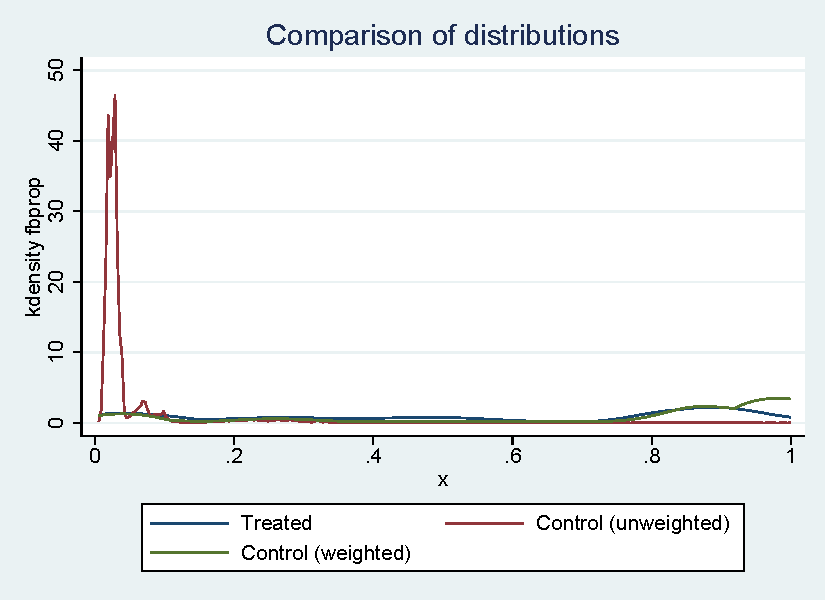
\includegraphics{797B_PS1_JL_7.pdf}
\end{center}
I compare matching based on different 
methods. I report each method's estimates in the table below. 
\newgeometry{left=1.5cm,bottom=0.1cm}
\begin{table}[htbp]\centering
\caption{Estimates of FB}
\begin{tabular}{l*{8}{c}}
\hline\hline
                    &   Bivariate&      Simple&   Saturated&         CEM&      PScore&   Psmatch\_1&         Own&         IPW\\
\hline
\hline
FB                  &      -0.056&       0.056&            &       0.050&      -0.077&       0.006&       0.125&       0.123\\
                    &     (0.011)&     (0.014)&            &     (0.015)&     (0.116)&     (0.032)&     (0.012)&     (0.142)\\
Obs.                &       51816&       51816&       48626&       37081&       65741&       51816&       51816&       51816\\
Estimator           &OLS Bivariate&OLS Controls&OLS Saturated&         CEM&       Match&       Match&       Match&       Match\\
\hline\hline
\multicolumn{9}{l}{\footnotesize Standard errors in parentheses}\\
\multicolumn{9}{l}{\footnotesize Average Treatment On Treated for matching models}\\
\end{tabular}
\end{table}

\restoregeometry

\end{document}

